
\usepackage{amsfonts}
\usepackage[dvips]{graphicx}
\usepackage[dvips]{epsfig}
\usepackage{fancyhdr}
\usepackage{dsfont}
\usepackage{amsmath}
\usepackage{dsfont}
\usepackage{amssymb}

%\usepackage{showkeys}
%\usepackage{showidx}

\usepackage{rotating}
\usepackage{shortvrb}
\usepackage{multicol}
\usepackage{longtable}
\usepackage{xr}

\usepackage[ps2pdf]{thumbpdf}
\usepackage[ps2pdf]{hyperref}

\input{prepictex}
\input{pictexwd}
\input{postpictex}

\hypersetup{
%    pdffitwindow=true,
    pdfstartview=FitB,
    pdftitle={BayesX Manuals},
    pdfauthor={Christiane Belitz, Andreas Brezger, Thomas Kneib, Stefan Lang and Nikolaus Umlauf},
    colorlinks=true,
    linkcolor=blue,
    pdfpagemode=UseOutlines,
    bookmarksopen=true,
    bookmarksnumbered=true,
    pdfstartpage={1},
    hyperindex=true
    }

\usepackage[dcu]{harvard}

\sloppy
\parindent0em
\parskip0.3em
\topmargin -0.3cm \textheight24cm \textwidth16.5cm \headheight0.5cm \oddsidemargin-0.4cm \evensidemargin-0.4cm

 \fancyhead[RO,LE]{\thepage}
 \fancyhead[C]{}
 \fancyhead[LO]{\nouppercase\rightmark}
 \fancyhead[RE]{\nouppercase\leftmark}
 \fancyfoot[RO,LE]{}
 \fancyfoot[C]{\small\today} %Am ende raus!!!
 \fancyfoot[LO,RE]{}
 \fancyfoot[C]{}

 \renewcommand{\headrulewidth}{.4pt}
 \renewcommand{\footrulewidth}{0pt} %Am Ende 0 !!!

\pagestyle{fancy}


\renewcommand{\descriptionlabel}[1]{\hspace\labelsep\sc #1}

 \newcommand{\Cov}{\mbox{Cov}}
 \newcommand{\diag}{\mbox{diag}}
 \newcommand{\trace}{\mbox{trace}}
 \newcommand{\df}{\mbox{df}}

\def \re {{\bf R}}
\def \beq {\begin{equation}}
\def \eeq {\end{equation}}
\def \bdis {\begin{displaymath}}
\def \edis {\end{displaymath}}
\def \ds {\displaystyle}

\def \mbeta {\mbox{\boldmath $\beta$}}
\def \mtheta {\mbox{\boldmath $\theta$}}
\def \hatmbeta {\mbox{\boldmath $\hat\beta$}}
\def \eps {\epsilon}
\def \meps {\mbox{\boldmath $\epsilon$}}
\def \mmu {\mbox{\boldmath $\mu$}}
\def \mnu {\mbox{\boldmath $\nu$}}
\def \mSigma {\mbox{\boldmath $\Sigma$}}
\def \mGamma {\mbox{\boldmath $\Gamma$}}
\def \msigma {\mbox{\boldmath $\sigma$}}
\def \mPhi {\mbox{\boldmath $\Phi$}}

\newcommand{\N}{\mbox{N}}
\newcommand{\Var}{\mbox{Var}}
\newcommand{\E}{\mbox{E}}

\newcommand{\X}{\mbox{\boldmath $X$}}
\newcommand{\x}{\xvec}
\newcommand{\Z}{\mbox{\boldmath $Z$}}
\newcommand{\z}{\mbox{\boldmath $z$}}
\newcommand{\mb}{\mbox{\boldmath $b$}}
\newcommand{\Fx}{\mbox{\scriptsize \boldmath $x$}}
\newcommand{\I}{\mbox{\boldmath $I$}}
\newcommand{\Y}{\mbox{\boldmath $Y$}}
\newcommand{\y}{\mbox{\boldmath $y$}}
\newcommand{\mS}{\mbox{\boldmath $S$}}
\newcommand{\T}{\mbox{\boldmath $T$}}
\newcommand{\K}{\mbox{\boldmath $K$}}
\newcommand{\kt}{\mbox{\boldmath $t$}}
\newcommand{\U}{\mbox{\boldmath $U$}}
\newcommand{\fu}{\mbox{\boldmath $u$}}
\newcommand{\ba}{\mbox{\boldmath $\alpha$}}
\newcommand{\bb}{\mbox{\boldmath $\beta$}}

\def \Mvec {\vec{M}}
\def \Kvec {\vec{K}}
\def \mM {\vec{M}}
\def \Pvec {\vec{P}}
\def \Svec {\vec{S}}
\def \deltavec {\vec{\delta}}
\def \lambdavec {\boldsymbol{\lambda}}
\def \Lambdavec {\boldsymbol{\Lambda}}
\def \betavec {\boldsymbol{\beta}}
\def \etavec {\boldsymbol{\eta}}
\def \gammavec {\boldsymbol{\gamma}}
\def \Gammavec {\boldsymbol{\Gamma}}
\def \Omegavec {\boldsymbol{\Omega}}
\def \muvec {\boldsymbol{\mu}}
\def \kappavec {\boldsymbol{\kappa}}
\def \nuvec {\boldsymbol{\nu}}
\def \pivec {\vec{\pi}}
\def \thetavec {\vec{\theta}}
\def \varthetavec{\vec{\vartheta}}
\def \varepsilonvec {\boldsymbol{\varepsilon}}
\def \zetavec {\vec{\zeta}}
\def \Sigmavec {\boldsymbol{\Sigma}}
\def \Thetavec {\boldsymbol{\theta}}

\def \dvec {\mathbf{d}}
\def \fvec {\mathbf{f}}
\def \fhatvec {\mathbf{\hat{f}}}
\def \svec {\mathbf{s}}
\def \wvec {\mathbf{w}}
\def \xvec {\mathbf{x}}
\def \yvec {\mathbf{y}}
\def \uvec {\mathbf{u}}
\def \avec {\mathbf{a}}
\def \zvec {\mathbf{z}}
\def \bvec {\mathbf{b}}
\def \tvec {\mathbf{t}}
\def \mvec {\mathbf{m}}
\def \cvec {\mathbf{c}}

\def \ds {\displaystyle}

\def \Gvec {\mathbf{G}}
\def \Rvec {\mathbf{R}}
\def \Avec {\mathbf{A}}
\def \Bvec {\mathbf{B}}
\def \Cvec {\mathbf{C}}
\def \Dvec {\mathbf{D}}
\def \Fvec {\mathbf{F}}
\def \Kvec {\mathbf{K}}
\def \Hvec {\mathbf{H}}
\def \Ivec {\mathbf{I}}
\def \Lvec {\mathbf{L}}
\def \Uvec {\mathbf{U}}
\def \Wvec {\mathbf{W}}
\def \Yvec {\mathbf{Y}}
\def \Zvec {\mathbf{Z}}
\def \svec {\mathbf{s}}
\def \Cvec {\mathbf{C}}
\def \dvec {\mathbf{d}}
\def \Avec {\mathbf{A}}
\def \Pvec {\mathbf{P}}
\def \Vvec {\mathbf{V}}
\def \xivec {\mathbf{x_i}}
\def \xjvec {\mathbf{x_j}}
\def \betavecr {\vec{\beta_r}}
\def \betadach {\hat{\vec{\beta}}}
\def \betadachr {\vec{\hat{\beta}_r}}
\def \betaschl {\vec{\tilde{\beta}}}
\def \betaschlr {\vec{\tilde{\beta}_r}}
\def \sschlr {\vec{\tilde{s}_r}}
\def \Aschlr {\vec{\tilde{A}_r}}
\def \Adach {\vec{\hat{A}}}
\def \Avecr {\vec{A}_r}
\def \Adachr {\vec{\hat{A}_r}}
\def \Fdach {\vec{\hat{F}}}
\def \Vdach {\vec{\hat{V}}}
\def \Aschl {\vec{\tilde{A}}}
\def \Xvec {\mathbf{X}}

\def \nullvec {\boldsymbol{0}}

\def \hvec {\vec{h}}
\def \vvec {\vec{v}}
\def \wvec {\vec{w}}
\def \x1vec {\vec{x_1}}
\def \xnvec {\vec{x_n}}

\def \Kmat {\mathbf{K}}
\def \Kmatj {\mathbf{K}_j}
\def \Xmat {\mathbf{X}}
\def \Vmat {\mathbf{V}}
\def \Smat {\mathbf{S}}

\def \einsvec {\boldsymbol{1}}

\newcommand{\subheader}[1]{\textsf{\textbf{{\large #1}}}}

\newenvironment{stanza}[2]{\subheader{#1} \begin{itemize} \item[]#2}{\end{itemize}}


\newcommand{\preface}[1]{
\thispagestyle{empty}

\begin{center}
{\bf \em \huge BayesX}

\vspace{0.5cm}

{\em \large Software for Bayesian Inference in Structured Additive Regression Models}

\vspace{0.5cm}

{\em Version 2.1}

\vspace{0.5cm}

\begin{figure}[h]
\begin{center}
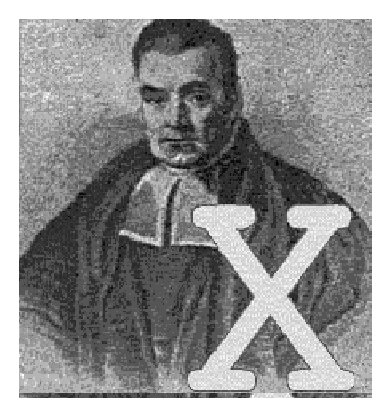
\includegraphics[scale=1.2]{grafiken/bayesicon.eps}
\end{center}
\end{figure}

\vfill

{\bf\sffamily \huge #1}

\vfill

\end{center}

{\em Developed by}

Christiane Belitz\\
Andreas Brezger\\
Thomas Kneib (University of G{\"o}ttingen)\\
Stefan Lang (University of Innsbruck) \\
Nikolaus Umlauf (University of Innsbruck) \\

\vspace{2ex}

{\em With contributions by}

\vspace{-1.5ex}

\begin{multicols}{2}
Daniel Adler
Eva-Maria Fronk\\
Felix Heinzl\\
Andrea Hennerfeind\\
Manuela Hummel\\
Alexander Jerak\\
Susanne Konrath\\
Petra Kragler\\
Cornelia Oberhauser\\
Leyre Est\'{\i}baliz Osuna Echavarr\'{\i}a\\
Daniel Saban\'{e}s Bov\'{e} \\
Achim Zeileis
\end{multicols}

{\em Supported by}

Ludwig Fahrmeir (mentally)\\
Leo Held (mentally)\\
German Research Foundation (DFG)

\newpage

\subsection*{Acknowledgements}

The development of {\em BayesX} has been supported by grants from the German Research Foundation (DFG), Collaborative
Research Center 386 ``Statistical Analysis of Discrete Structures''.

Special thanks go to (in alphabetical order of first names):

{\em Dieter Gollnow} for computing and providing the map of Munich (a really hard job); \\
{\em Leo Held} for advertising the program; \\
{\em Ludwig Fahrmeir} for his patience with finishing the program and for carefully
reading and correcting the  manual; \\
{\em Ngianga-Bakwin Kandala} for being the first user of the program (a really hard job); \\
{\em Samson Babatunde Adebayo} for carefully reading and correcting the manual; \\
{\em Ursula Becker} for carefully reading and correcting the manual;

\subsection*{Licensing agreement} 

This program is free software; you can redistribute it and/or
modify it under the terms of the GNU General Public License
as published by the Free Software Foundation; either version 2
of the License, or (at your option) any later version.

This program is distributed in the hope that it will be useful,
but WITHOUT ANY WARRANTY; without even the implied warranty of
MERCHANTABILITY or FITNESS FOR A PARTICULAR PURPOSE.  See the
GNU General Public License for more details.

You should have received a copy of the GNU General Public License
along with this program; if not, write to the Free Software
Foundation, Inc., 51 Franklin Street, Fifth Floor, Boston, MA  02110-1301, USA. 



\vspace{0.5cm}

{\em BayesX} is available at { \href{http://www.bayesx.org}{http://www.bayesx.org}}}
